\documentclass{article}

\usepackage{graphicx, caption, subcaption}
\usepackage{amsmath, amsfonts, amsthm}
\usepackage{algorithm, algpseudocode}

\usepackage{hyperref}
\hypersetup{
    colorlinks,
    citecolor=black,
    linkcolor=black,
    urlcolor=blue
}

\newtheorem*{theorem}{Theorem}

% Automatic float-barrier around subsections
\usepackage[section]{placeins}
\makeatletter
\AtBeginDocument{%
  \expandafter\renewcommand\expandafter\subsection\expandafter{%
    \expandafter\@fb@secFB\subsection
  }%
}
\makeatother

\setcounter{tocdepth}{2}

\begin{document}

\title{A Gentle Introduction to Elliptic Curve Cryptography}
\author{Tanner Prynn}
\maketitle

\tableofcontents
\clearpage

%\section*{Foreword}
%\addcontentsline{toc}{section}{Foreword}
%Draft of project for Math 415B.
%
%Status of code: complete. See \texttt{curve25519.rb}.
%
%Status of problems: incomplete. See \texttt{problems.pdf}.
%
%Status of report: incomplete. Outline completed with some sections filled in.
%
%In writing this report, I aimed to hit the most important points for a picture of elliptic curves as they would be applied for cryptography. 
%Some sections are (or will be) rigorous while others simply provide an overview or guided discussion of ``why things are the way they are''. 
%The references provide a much more in-depth discussion of this topic.
%
%Sections I've omitted that I could include: Projective Geometry, Finite Field Arithmetic, Derivation of Group Law for Montgomery Curves
%
%Sections I've included that I could omit: Normal Forms for Elliptic Curves/Acceptable Changes of Variables, Pohlig-Hellman Algorithm
%
%\clearpage

\section{Elliptic Curves}
An \textbf{elliptic curve} is a set of points satisfying an equation of the form
$$y^2 = x^3 + ax + b$$
for coefficients $a,b$ and variables $x,y$ in some field $F$ (of characteristic not 2 or 3). 
We place one additional restriction on an elliptic curve, which is that
$4a^3 + 27b^2 \neq 0$.
This condition ensures that the curve is \textit{non-singular}, which allows us to find a tangent line to any point on the curve \cite[$\S$3.1]{ecc-guide}.

Let's start with a few examples of curves, plotted over the real numbers.
Figure \ref{fig:ec-plot} shows a simple elliptic curve.
The three points where it crosses the $x$-axis correspond to the zeroes of the polynomial $x^3 - 3x + 1$.
Figure \ref{fig:ec-plot2} shows the elliptic curve $y^2 = x^3 - 2x + 2$, which only crosses the $x$-axis once in $\mathbb{R}$.

\begin{figure}[h]
\centering
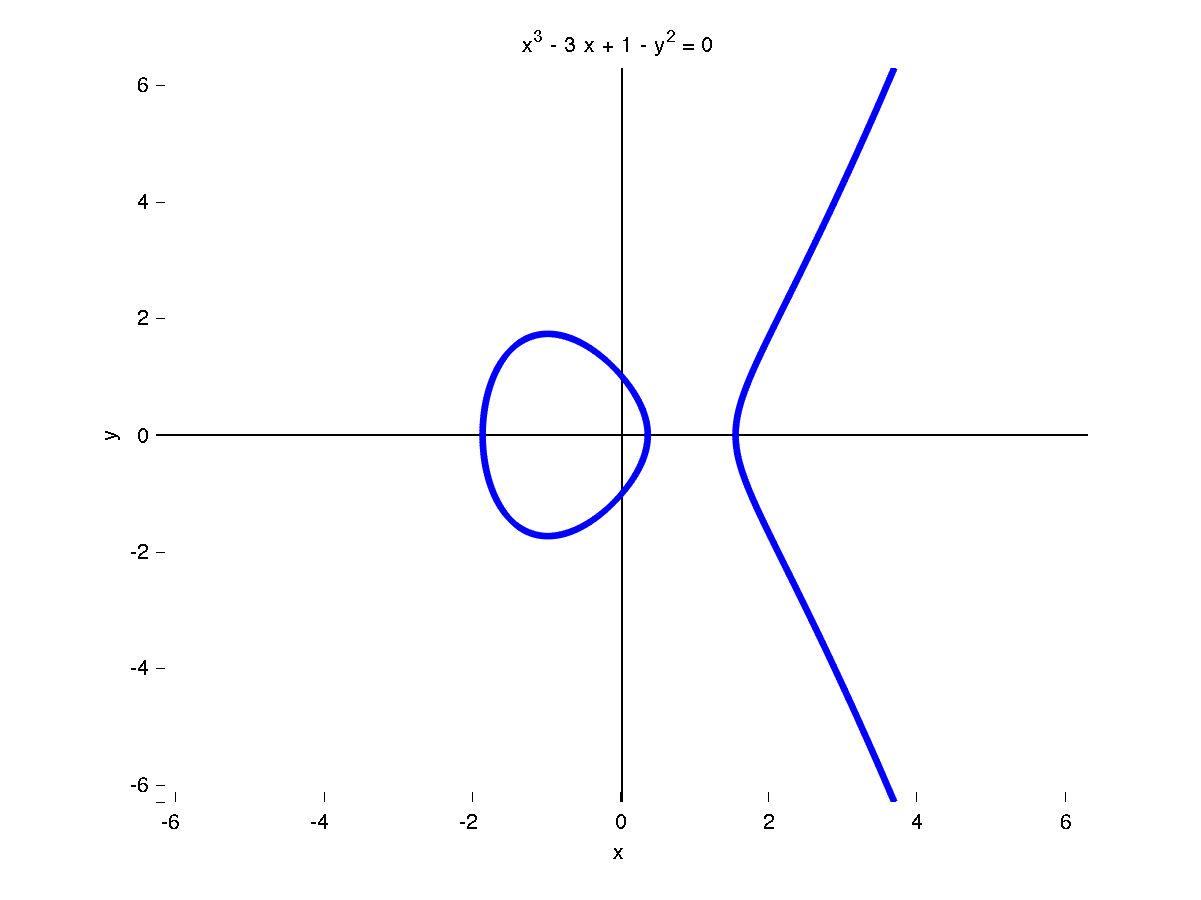
\includegraphics[width=\textwidth]{images/ec1.png}
\caption{The elliptic curve $y^2 = x^3 - 3x + 1$}
\label{fig:ec-plot}
\end{figure}

\begin{figure}[h]
\centering
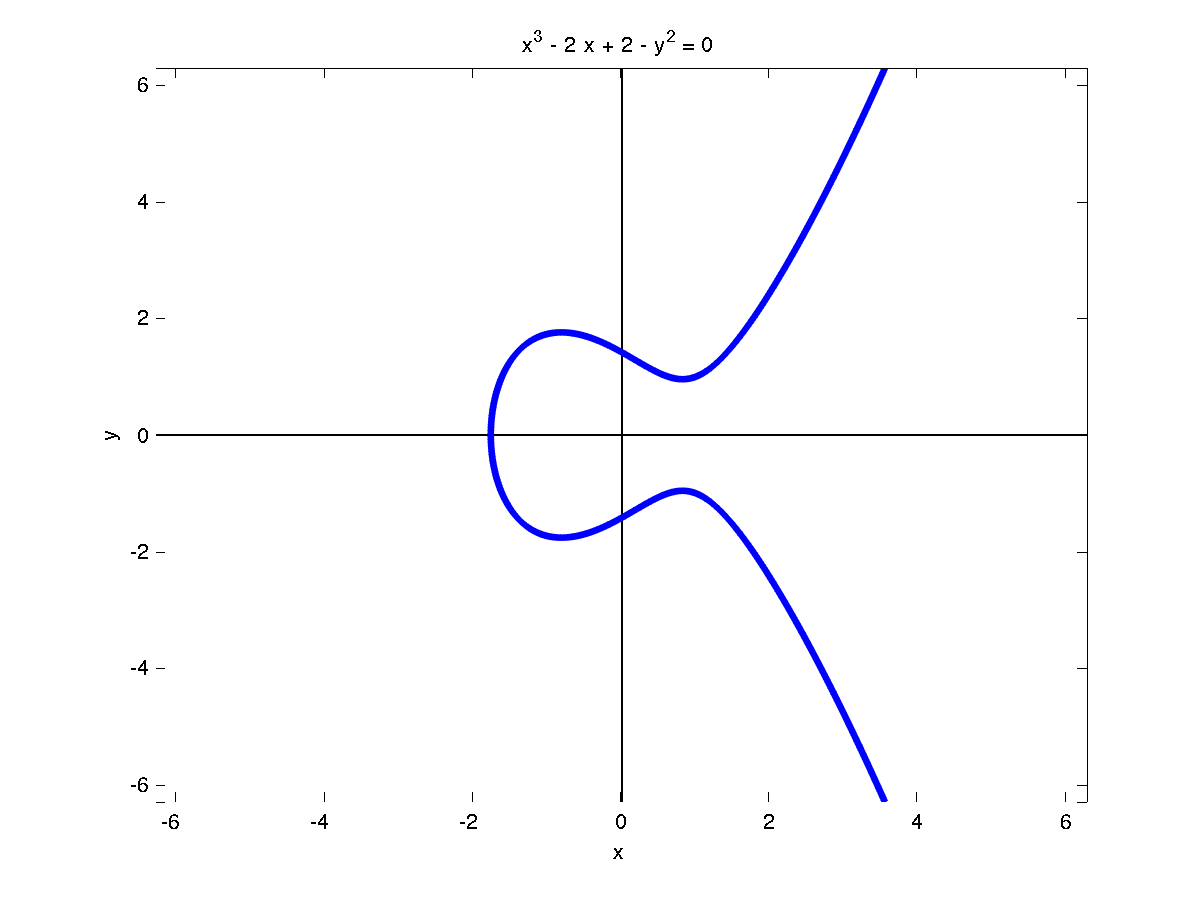
\includegraphics[width=\textwidth]{images/ec4g.png}
\caption{The elliptic curve $y^2 = x^3 - 2x + 2$}
\label{fig:ec-plot2}
\end{figure}

Figure \ref{fig:ec-singular} shows two singular curves.
To define a group operation on the points of the curve, we need to be able to take a tangent line to each point.
So we avoid these cases with that additional restriction on the coefficients.

\begin{figure}[h]
\centering

\begin{subfigure}{.5\textwidth}
	\centering
	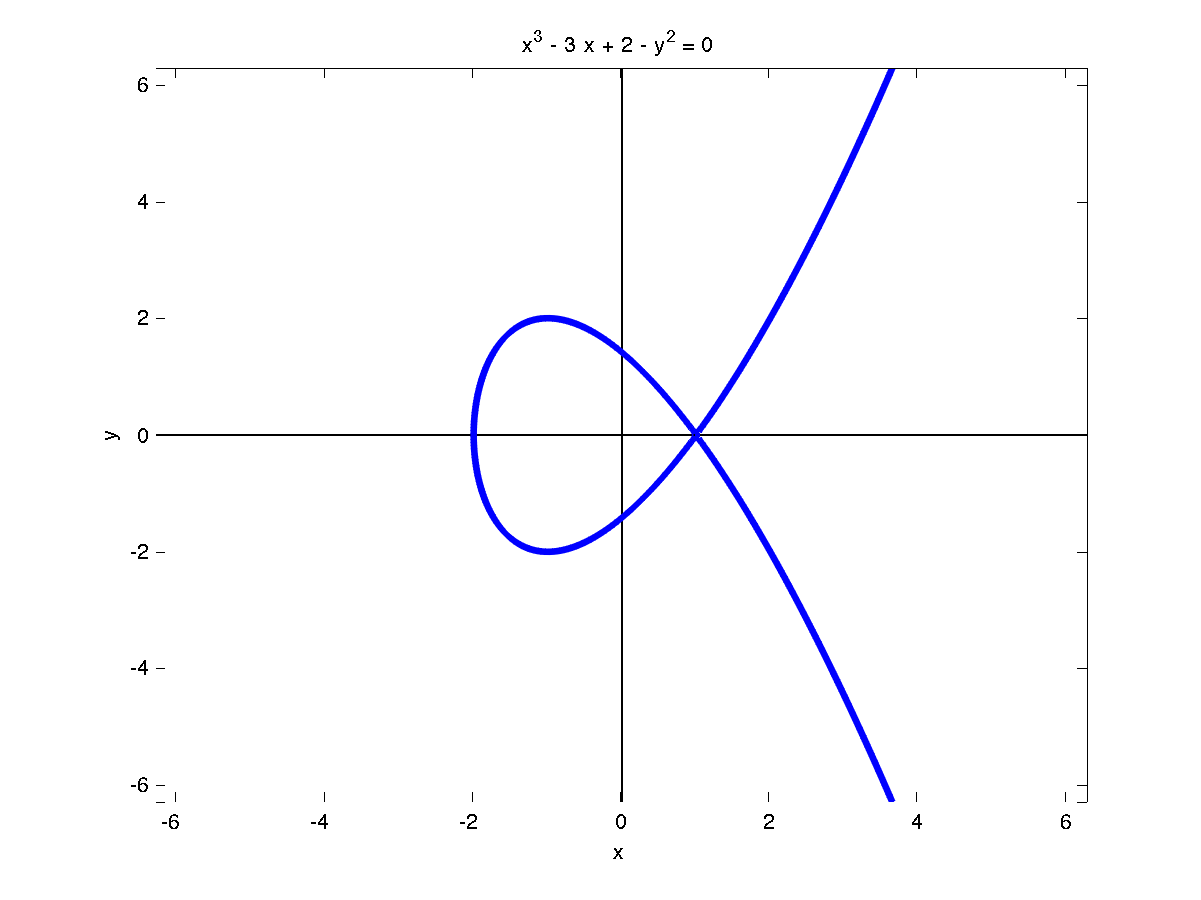
\includegraphics[width=1\linewidth]{images/ec2.png}
	\caption{The curve $y^2 = x^3 - 3x + 2$}
\end{subfigure}%
~%
\begin{subfigure}{.5\textwidth}
	\centering
	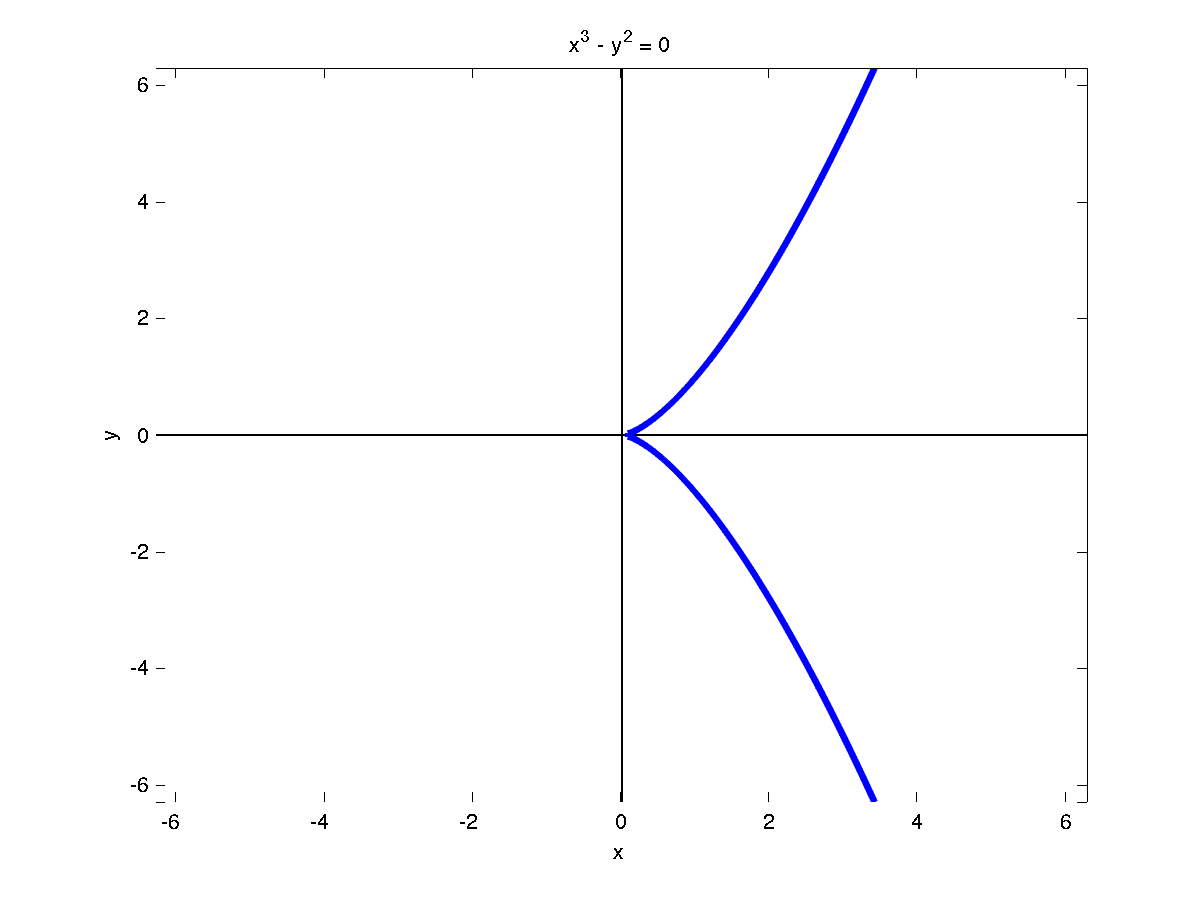
\includegraphics[width=1\linewidth]{images/ec3.png}
	\caption{The curve $y^2 = x^3$}
\end{subfigure}

\caption{These curves have a `singularity': a point where the tangent is not clearly defined.}
\label{fig:ec-singular}
\end{figure}

\subsection{Defining a Group Operation}
Now, we have an equation for a curve, and we can define the set of points 
$$C = \{(x,y) \mid x,y \in F \text{ and } y^2 = x^3 + ax + b\}$$
which is a subset of of the plane $F^2$.
We want to make the set $C$ into a group, so we need to define an operation on it.
Let's call that operation $*$, and we'll define $P_1 * P_2$ as the third intersection of the line through $P_1$ and $P_2$ which lies on the curve $C$.
Figure \ref{fig:ec-3rd-intersection} shows this operation for the simple case of two different points.

\begin{figure}[h]
\centering
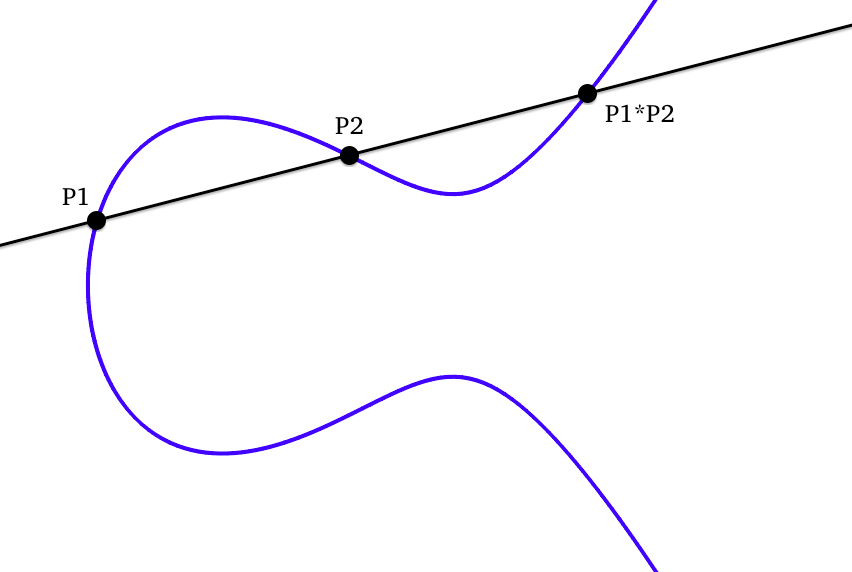
\includegraphics[width=0.6\textwidth]{images/ec4-star.png}
\caption{Finding the third point of intersection on the curve $y^2 = x^3 - 2x + 2$}
\label{fig:ec-3rd-intersection}
\end{figure}

What other cases are there?
First, we need to define $*$ when $P_1 = P_2$.
We want to have the line through $P_1$ hit the curve at exactly two points, $P_1$ and $P_1*P_1$.
To achieve this, let the line through $P_1$ be the tangent to the curve.
Then the tangent line intersects the curve at one additional point, as desired (figure \ref{fig:ec-tangent}) \cite[$\S$I.2]{rational-points}.

\begin{figure}[h]
\centering
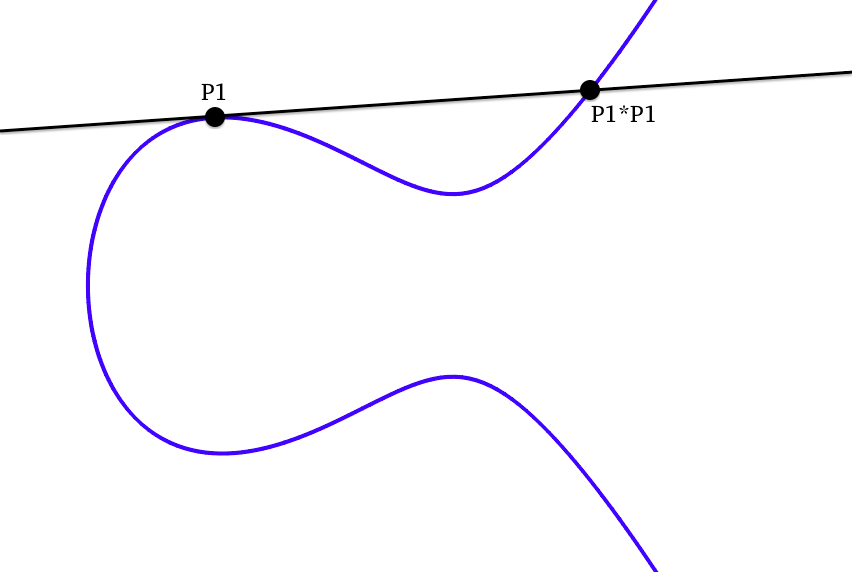
\includegraphics[width=0.6\textwidth]{images/ec4-tangent.png}
\caption{A tangent line intersects the curve at two points.}
\label{fig:ec-tangent}
\end{figure}

Now, we come to the case of a vertical line.
A vertical line will intersect our curve at exactly two points, because the curve is symmetric over the $x$-axis.
But those two points will violate our $*$ operation, because there isn't a third-point where the line intersects the curve (figure \ref{fig:ec-infinity}).
This leads us to take an idea from projective geometry: that there is an extra point on the curve called the \textit{point at infinity}.

\begin{figure}[h]
\centering
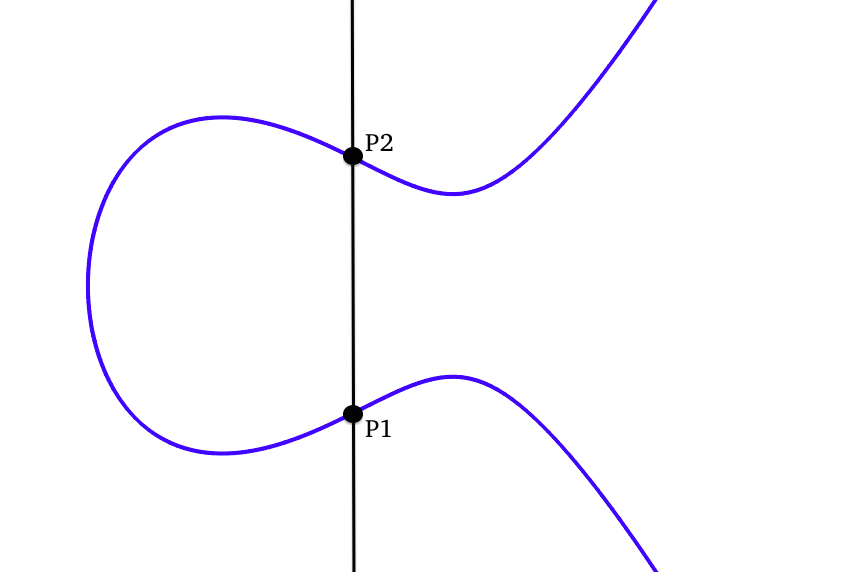
\includegraphics[width=0.6\textwidth]{images/ec4-infinity.png}
\caption{A vertical line only intersects the curve at two points.}
\label{fig:ec-infinity}
\end{figure}

The point at infinity (denoted $\infty$) is a point in the projective plane, so there isn't an intuitive way to draw it in our standard plane.
However, we can understand $\infty$ as `outside' of the plane, and simply treat it as a special geometric object.
As a benefit, we can take the third intersection of a vertical line to be $\infty$.
We then need to redefine the set of points $C$ to include $\infty$:
$$C = \{\infty\} \cup \{(x,y) \mid x,y \in F \text{ and } y^2 = x^3 + ax + b\}$$
Thus we have disposed of this problematic case \cite[$\S$2.2]{washington}.

Having $\infty$ on our curve is also useful because it is a unique point which exists on every elliptic curve.
This makes it an ideal candidate for the identity element of our group operation.
We need to redefine our operation to make this true, however.
If we reconsider the case of the vertical line, we have two points $P_1$ and $P_2$ such that $P_1 * P_2 = \infty$.
Because the curve is symmetric, all we need to do to get $P_1$ from $P_2$ is to reflect over the $x$-axis.

Let's define a new operation $+$ and say that, for any point $P \in C$, $P = P+\infty = \infty+P$.
To produce $+$ from our previous operation $*$, we only need to add one additional step: a reflection over the $x$-axis.
We will see later that this operation is commutative, which is why we chose to use the addition symbol \cite[$\S$2.2]{washington}.
Figure \ref{fig:ec-plus} revisits the previous cases to show how this new operation works.

\begin{figure}[h]
\centering

\begin{subfigure}{.5\textwidth}
	\centering
	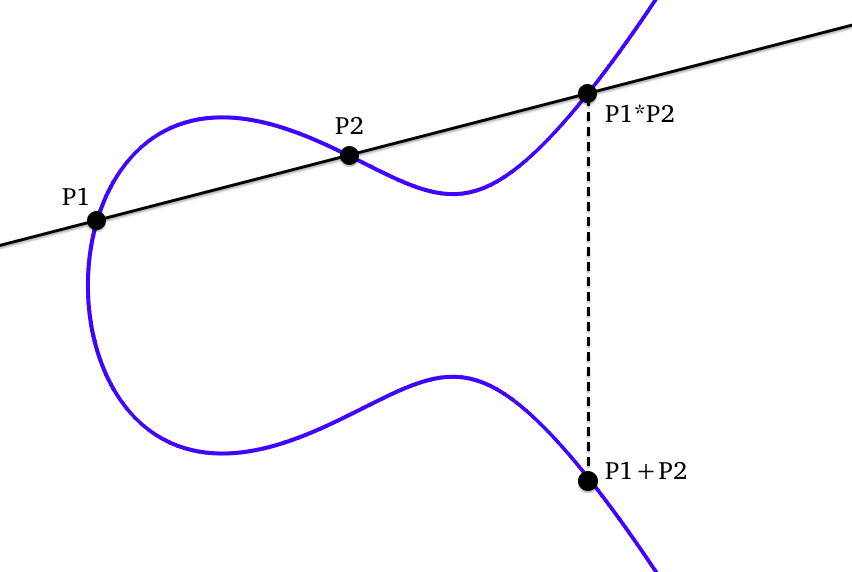
\includegraphics[width=1\linewidth]{images/ec4-plus.png}
	\label{fig:ec-plus-1}
\end{subfigure}%
~%
\begin{subfigure}{.5\textwidth}
	\centering
	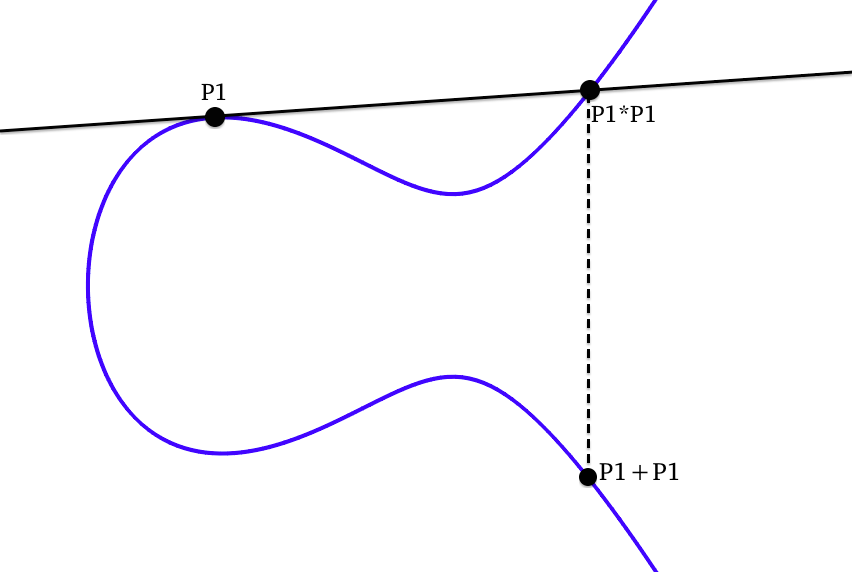
\includegraphics[width=1\linewidth]{images/ec4-plus-tangent.png}
	\label{fig:ec-plus-2}
\end{subfigure}

\caption{The $+$ operation for two points on an elliptic curve}

\label{fig:ec-plus}
\end{figure}

\subsection{Deriving the Group Law}
Now that we have defined the group operation geometrically, we can derive a formula for it.

\subsubsection{Identity}
Define $\infty$ to be the identity. For any point $P$ on $C$, $P+\infty = \infty + P = P$.

\subsubsection{Addition}
Let $P_1 = (x_1,y_1), P_2 = (x_2,y_2)$ on $C$ with $P_1 \neq P_2$.
If $x_1 = x_2$, then the line is vertical and we define $P_3 = \infty$.
Otherwise, the equation of the line through $P_1$ and $P_2$ has the form $y = mx + b$, where $m = \frac{y_2-y_1}{x_2-x_1}$ and $b = y_1 - mx_1$.
Now substitute this into the equation of our curve to obtain
$$(mx+b)^2 = x^3 + ax + b$$
Expand and rewrite to get a cubic equation in $x$
$$0 = x^3 - m^2x^2 + (a-2mb)x + b - b^2$$
We know that this equation has three roots (of which we know two), so it must be equal to
$$0 = (x-x_1)(x-x_2)(x-x_3)$$
Multiplying out, we find that the coefficient of the $x^2$ term has the form $-x_1 - x_2 - x_3$. So $-m^2 = -x_1 - x_2 - x_3$, and we can solve for the third x-coordinate in terms of the first two points:
$$x_3 = m^2 - x_1 - x_2$$
Finally, the third point is reflected across the x-axis.
To find the y-coordinate, we substitute our x-coordinate in to the equation of our line and negate it.
$$y_3 = -(mx_3 + b)$$.

\subsubsection{Doubling}
Let $P_1$ on $C$.
We defined the addition of a point with itself by taking the tangent line to that point on the curve.
We can find the slope of the tangent line by implicit differentiation:
\begin{align*}
2y \frac{dy}{dx} &= 3x^2 + a \\
\frac{dy}{dx} &= \frac{3x^2+a}{2y} \\
m &= \frac{dy}{dx}(x_1,y_1) 
\end{align*}
Then we simply follow the same process for addition.
\begin{align*}
x_2 &= m^2 - 2x_1 \\
y_2 &= -(mx_1 + b)
\end{align*}

\subsubsection{Inverses}
Let $P=(x,y)$ on $C$. Define $-P = (x,-y)$.
The line through $P$ and $-P$ is vertical, and hence intersects the curve at $P$, $-P$, and $\infty$.
$\infty$ is a unique point on our curve, and has the special property that ``reflecting across the x-axis'' (negating the y-coordinate) returns $\infty$.
So $P + (-P) = \infty$.

\subsubsection{Closure}
Now we have fully defined the group law for an elliptic curve.
The closure of the set $\{\infty\} \cup \{(x,y) \mid x,y \in F \text{ and } y^2 = x^3 + ax + b\}$ follows from the group law and the closure of the field $F$.

\subsubsection{Commutativity}
The group law is commutative because the line through two points is defined symmetrically.
In other words, the line through points $A$ and $B$ is the same as the line through points $B$ and $A$.

\subsubsection{Associativity}
We will prove the associativity of the group law geometrically, but it also follows algebraically from the formulas above.
To complete the proof, we will use a theorem from projective geometry:

\begin{theorem}[Cayley-Bacharach Theorem]
Let $C$, $C_1$, and $C_2$ be three cubic curves.
Suppose $C$ goes through eight of the nine points of $C_1$ and $C_2$.
Then $C$ goes through the ninth intersection point.
\end{theorem}

Let $P,Q,R$ on our elliptic curve $E$.
To show that $P+(Q+R) = (P+Q)+R$, it suffices to show that $P*(Q+R) = (P+Q)*R$.
Our goal is to define two cubic curves, one of which intersects $P*(Q+R)$ and the other which intersects $(P+Q)*R$.
Then, if their other eight points of intersection match, it must be that $P*(Q+R) = (P+Q)*R$.

Let $C_1$ be the curve through $P*(Q+R)$ and $C_2$ the curve through $(P+Q)*R$.
We will construct $C_1$ and $C_2$ directly.
Consider a linear equation $f(x,y) = ax + by + c = 0$.
Given three such equations $f_1, f_2, f_3$, we can construct a cubic curve $g(x,y) = (f_1(x,y))(f_2(x,y)(f_3(x,y)) = 0$.
Then every zero of $g$ is on one of the lines; so the curve is the union of the points on each of the lines and the point at infinity.

Let's start with $C_1$ (figure \ref{fig:ec-assoc-1}).
We want to deconstruct the point $P*(Q+R)$ into three linear equations.
The first line is the line between $Q$ and $R$, whose third point of intersection is $Q*R$.
The second line is between $Q*R$ and $\infty$, which intersects the curve at $Q+R$.
The third line is between $Q+R$ and $P$, which intersects the curve at $P*(Q+R)$.

\begin{figure}[h]
\centering
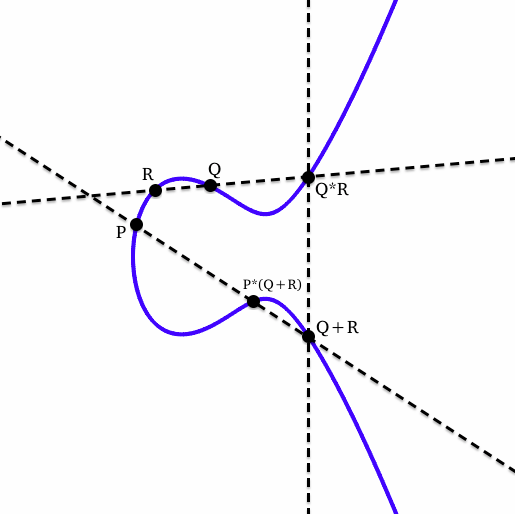
\includegraphics[width=0.8\linewidth]{images/ec5-assoc-1.png}
\caption{Defining $C_1$ as the union of three lines}
\label{fig:ec-assoc-1}
\end{figure}

For $C_2$, we define the lines similarly (figure \ref{fig:ec-assoc-2}).
Line one has intersections $P$, $Q$, and $P*Q$.
Line two has intersections $P*Q$, $\infty$, and $P+Q$.
Line three has intersections $P+Q$, $R$, and $P*(Q+R)$.
Thus we have two curves $C_1$ and $C_2$ which intersect at eight points, so their ninth point of intersection is equal by Cayley-Bacharach.
\cite[\S 1.2]{rational-points}

\begin{figure}[h]
\centering
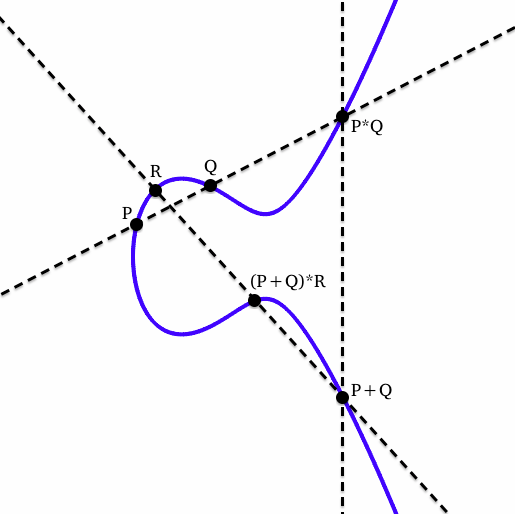
\includegraphics[width=0.8\linewidth]{images/ec5-assoc-2.png}
\caption{Defining $C_2$ as the union of three lines}
\label{fig:ec-assoc-2}
\end{figure}

This completes our proof that $(E,+)$ is a group.

\subsection{Weierstrass Form and Acceptable Changes of Variables}
General form of a cubic curve.
Weierstrass Form is not the `only' form of an elliptic curve. 
We can use an acceptable changes of variables/biration equivalence to write other forms of elliptic curves.

E.g. Montgomery Curve

\clearpage

\section{The Discrete Logarithm Problem}
Given a group $G$ with operation $*$ we can define a map $\cdot: \mathbb{Z} \times G \to G$ by
$$n\cdot g \mapsto \underbrace{g * g * \cdots * g}_{n\text{ times}}$$

Let's first consider the case of $\mathbb{Z}_p^*$, the multiplicative group of integers mod $p$.
In this case, our map $\cdot$ is equivalent to exponentiation.
Let $a,b \in \mathbb{Z}_p^*$ and assume $\exists n \in \mathbb{Z}$ such that $a^n = b$.
Over the real numbers, we call solving for $n$ finding a logarithm. Over $\mathbb{Z}_p^*$, $n$ is the \textit{discrete logarithm} of $b$ with respect to the base $a$.

For an elliptic curve $C$, we also have a group structure. 
In this case, the map $\cdot$ is equal to the repeated addition of a point to itself. 
We can call this map \textit{point multiplication}.
For a point $P$ on $C$, $nP = P + P + \cdots + P$.
Again, there is an analogue to the logarithm.
If we have two points $P,Q$ on $C$ where $nP = Q$, then $n$ is the \textit{elliptic-curve discrete logarithm} (ECDL) of $Q$ with respect to $P$.

\subsection{Trap-Door Functions}
Why do we bother defining such a simple operation?
It turns out that this is the exact operation we will use to construct a cryptosystem.
In fact, many modern cryptosystems are based on a class of operations called \textit{trap-door functions}.
A trap-door function is a function that is simple to compute in one direction, but very costly to compute in the other direction.
In the case of the ECDL, it is simple to compute a point multiplication, but hard to compute the logarithm.

Note that this is not a formal definition.
In general, a trap-door function is infeasible to break, given current computing resources.
However, most trap-door functions can only be conjectured to be secure.
While we currently do not know any algorithms which solve the ECDLP, there is no guarantee that a fast algorithm does not exist.
Next, we'll consider a basic approach to solving ECDLP.

\subsection{Attacks on Discrete Logarithms}
Imagine we're playing a game.
I pick a point $P$ on an elliptic curve, and tell you the curve's parameters and the point I picked.
Then I pick a secret integer $s$ and tell you $sP$. Your job is to find $s$.
This is the basic model of a user and attacker in cryptosystem which is based on the ECDL.
Given $P$ and $sP$, can the attacker find $s$? Let's look at how the attacker might go about doing that.

\subsubsection{Naive Multiplication}
Our first attempt will be to simply try every integer $k$.
If $kP = sP$ then we know $k = s$.
If our curve has only a small number of points, then a computer will chew through this problem in seconds.
Let's say our curve has $N$ points, and each point multiplication takes a maximum of $M$ operations.
Then naive multiplication has algorithmic complexity $O(NM)$.

From a user's perspective, $M$ should be small, so curve operations are fast.
In order to make the attacker's life difficult, $N$ should be large: the chosen curve should have a large number of points.
Many curves used for cryptography are over large prime fields, with a massive number of points (more than $2^{200}$).
Using a naive algorithm against such a curve, even with an extremely fast computer, probably won't finish in our lifetime.

\subsubsection{Baby Step Giant Step}
There are a number of algorithms which reduce the amount of time it takes to solve the ECDLP.
Let's consider an elliptic curve (or a subgroup) which is cyclic, with generator $G$ and order $N$.
The user picks $n$ and computes $nG$. 

The Baby-Step Giant-Step algorithm rewrites the point $P = nG$ as $(im + j)G$, with $m = \lceil \sqrt{N} \rceil$.
Then $jP$ is computed for $0 \leq j < m$ and stored.
Finally, multiplication is used to find $imG$ for $0 \leq i < m$, which is subtracted from $P$ to solve for $jG$.

\begin{algorithm}
\caption{Baby-Step Giant-Step for ECDLP}
\begin{algorithmic}
\State $m \gets \sqrt{N}$
\For{$0 \leq j < m$}
	\State Compute and store $(j, jP)$
\EndFor
\For{$0 \leq i < m$}
	\State Compute $Q - imP$
	\If{$Q-imP = jP$ for some $j$}
		\State \Return $n \equiv j + im$
	\EndIf
\EndFor
\end{algorithmic}
\end{algorithm}

Baby-Step Giant-Step completes in $O(\sqrt{N} M)$ time and $O(\sqrt{N})$ space complexity.
This is a large improvement over naive multiplication, but still very slow on cryptographic curves. 
While there are some algorithms which solve specific cases of the ECDLP, there is no known algorithm which feasibly solves this problem on a general cryptographic curve.
The security of an elliptic curve cryptosystem relies on this fact \cite[\S 5]{washington}.

\clearpage

\section{Elliptic-Curve Diffie-Hellman Exchange}
The split between what we recognize as modern and pre-modern cryptography coincides directly with the development of public key cryptography.
Public key cryptography is a class of cryptosystems which are defined by the fact that each user has a public key, which they publish for anyone to see, and a private key, which they keep secret.
The public key allows anyone who wants to communicate with that user to derive some information which is only shared between those two users, even over an insecure channel.

One of the major problems of pre-modern cryptography was that every method of communication required a shared key.
This problem is called the key distribution problem.
Essentially, if two parties wanted to communicate they needed to meet and exchange a key - there was no way to communicate over an insecure channel without first communicating over a secure channel.
Public key cryptography solves this problem by allowing two parties to communicate without the need of a shared key, or to securely derive one over an insecure channel.

\subsection{The Diffie-Hellman Key Exchange}
The Diffie-Hellman Key Exchange is a method of key derivation which allows two users to derive a shared key over an insecure channel.
It is typical of cryptography to define communication algorithms as follows: imagine two users, Alice and Bob.
Alice and Bob want to communicate securely, but can only talk over an insecure line.
Somewhere on the insecure line an attacker, Eve, is listening in and attempting to decrypt their communication.

The \textbf{Elliptic Curve Diffie-Hellman Exchange} (ECDHE) proceeds as follows:
\begin{algorithm}
\caption{Elliptic Curve Diffie-Hellman Exchange}
\begin{enumerate}
\item Alice and Bob agree on a curve $C$ and a generating point $P$. (In practice, these parameters are standardized and known to everyone.)
\item Alice generates a random, secret integer $a$ and sends Bob $aP$.
\item Bob generates a random, secret integer $b$ and sends Alica $bP$.
\item Alice computes $a(bP)$.
\item Bob computes $b(aP)$.
\item Alice and Bob now share the key $abP$.
\end{enumerate}
\end{algorithm}

At this point, it is clear that Alice and Bob share the point $abP$.
Eve, however, only knows the points $aP$ and $bP$, which she cannot use to compute $abP$.
Thus for Eve to break the ECDHE, she must solve the ECDL: given $aP$, find $a$, or given $bP$, find $b$.
From now on, Alice and Bob can use a symmetric encryption algorithm (such as AES) to communicate securely.
Their shared key is derived from $abP$.
Note that $abP$ is a point on a curve, while most encryption algorithms desire keys to be a string of random bytes.
Typically Alice and Bob will use an agreed upon method of key derivation, such as a hash of the $x$-coordinate, to generate the actual session key \cite[\S 6.2]{washington}.

\subsection{Implementation Details of ECDH}

\subsubsection{Choice of Curve}
We now have all of the necessary information to implement a theoretical cryptosystem.
However, one of the most important choices in cryptographic design is the choice of parameters: what curve will we use, over what field, and what will the generating point be?
Wrong choices in these areas can result in massive holes in the security of the ECDL.
Daniel J. Bernstein and Tanja Lange have produced a \href{http://safecurves.cr.yp.to/}{database} of the numerous choices of curves, and how seemingly safe choices can be insecure.

For our implementation, we will use Bernstein's \textit{Curve25519}.
Curve25519 is an elliptic curve in Montgomery form, over the prime field $\mathbb{Z}_p$ where $p = 2^{255} - 19$.
This curve was designed for security: for example, it is not vulnerable to attacks based on subgroups of the curve \cite{curve25519}.

\subsubsection{Point Multiplication}
One consideration that is not very important in theory, but extremely important in reality is how to perform a point multiplication.
The naive method is to compute $nP$ by summing $n$ copies of $P$: $P + P + \cdots + P$.
This algorithm is exponential, which is to say, extremely slow for a real-world application.
We can see an immediate improvement from the decomposition of $n$ into binary.
Then, each zero bit of $n$ corresponds to a doubling of the point $P$, and each one bit of $n$ corresponds to adding $P$ and doubling.

Let $b_m b_{m-1} \cdots b_1 b_0$ be the binary representation of $n$ (where $b_m$ is the most-significant bit).
The Double-and-Add algorithm is described below.
\begin{algorithm}
\caption{Elliptic Curve Point Multiplication: Double-and-Add}
\begin{algorithmic}
\State $Q \gets \infty$
\For{$0 \leq i \leq m$}
	\If{$b_i = 1$}
		\State $Q \gets Q + P$
	\EndIf
	\State $Q \gets 2Q$
\EndFor
\State \Return $Q$
\end{algorithmic}
\end{algorithm}

While Double-and-Add is much faster than repeated addition, it demonstrates one of the difficulties of real-world cryptography.
Specifically, this algorithm leaks information about $n$ by performing a different number of doublings and additions based on the binary representation of $n$.
This information leakage makes an implementation which uses Double-and-Add vulnerable to timing or power analysis.
To avoid this vulnerability in practice, an ECDHE implementation will use the \href{http://safecurves.cr.yp.to/ladder.html}{Montgomery Ladder}, a multiplication algorithm which operates in constant time \cite[\S 3.3]{ecc-guide}. 

\clearpage

\begin{thebibliography}{9}

\bibitem{curve25519}
	Daniel J. Bernstein:
	\emph{Curve 25519: new Diffie-Hellman speed records}.
	Published \href{http://cr.yp.to/ecdh/curve25519-20060209.pdf}{online},
	2006.

\bibitem{ecc-guide}
	Darrel Hankerson, Alfred J. Menezes, and Scott Vanstone:
	\emph{Guide to Elliptic Curve Cryptography}.
	Springer,
	2004.

\bibitem{rational-points}
	Joseph Silverman and John Tate:
	\emph{Rational Points on Elliptic Curves}.
	Springer,
	1994.

\bibitem{washington}
	Lawrence Washington:
	\emph{Elliptic Curves: Number Theory and Cryptography}.
	Chapman and Hall/CRC,
	2nd edition,
	2008.

\end{thebibliography}

\end{document}